%%%%%%%%%%%%%%%%%%%%%%%%%%%%%%%%%%%%%%%%%%%%%%%%%%%%%%%%%%%%%%%%%%%%%%%%
%                                                                      %
% LaTeX, FIIW thesis template                                          %
% 28/11/2014 v1.2                                                      %
%                                                                      %
%%%%%%%%%%%%%%%%%%%%%%%%%%%%%%%%%%%%%%%%%%%%%%%%%%%%%%%%%%%%%%%%%%%%%%%%
\documentclass[11pt,a4paper]{report}
% Indien je je thesis recto-verso wil afdrukken gebruik je onderstaande opties i.p.v. bovenstaande
%\documentclass[11pt,a4paper,twoside,openright]{report}

\usepackage[a4paper,left=3.5cm, right=2.5cm, top=3.5cm, bottom=3.5cm]{geometry}
\usepackage[dutch]{babel}
\usepackage{graphicx}
\usepackage[latin1]{inputenc}           % om niet ascii karakters rechtstreeks te kunnen inputten
%\usepackage[utf8]{inputenc}            % commentarieer deze regel uit als je utf8 encoded files gebruikt in plaats van latin1
\usepackage{natbib}
\usepackage{listings}             		% voor het weergeven van broncode
\usepackage{verbatim}					% weergeven van code, commando's, ...
\usepackage{hyperref}					% maak PDF van de thesis navigeerbaar
\usepackage{url}						% URL's invoegen in tekst met behulp van \url{http://}
\usepackage[small,bf,hang]{caption}     % om de captions wat te verbeteren
\usepackage[final]{pdfpages}            % gebruikt voor het invoegen van het artikel in pdf-formaat
\usepackage{pslatex}					% andere lettertype's dan de standaard types
\usepackage{lipsum}
\usepackage{sectsty}					% aanpassen van de fonts van sections en chapters
%\usepackage[nottoc,numbib]{tocbibind}	% Bibliography mee in de ToC

\allsectionsfont{\sffamily}
\chapterfont{\raggedleft\sffamily}

\usepackage{float}                      % De optie H voor de plaatsing van figuren op de plaats waar je ze invoegt. bvb. \begin{figure}[H]
%\usepackage{longtable}					% tabellen die over meerdere pagina's gespreid worden
%\usepackage[times]{quotchap}           % indien je fancy hoofdstuktitels wil
%\usepackage[none]{hyphenat}
%\usepackage{latexsym}
%\usepackage{amsmath}
%\usepackage{amssymb}

% MFA: zet zoekpad voor figure
\graphicspath{{fig/}}

\usepackage{fiiw}
% \usepackage{fiiw_denayer_eng} % For the english version (also change last page at the bottom of this file!

%door onderstaande regels in commentaar te zetten, of op false, kan je pagina's weglaten
%bijvoorbeeld het weglaten van een voorwoord, lijst met symbolen, ...
%%%%%%%%%%%%%%%%%%%%%%%%%%%%%%%%%%%%%%%%%%%%%%%%%%%%%%%%%%%%%%%%%%%%%%%%%%%%%%%%%%%%%%%%
%voorwoord toevoegen?
\acknowledgementspagetrue
\acknowledgements{voorwoord}			%.tex file met daarin het voorwoord

%samenvatting toevoegen
\summarypagetrue
\summary{samenvatting}					%.tex met daarin de samenvatting

%abstract toevoegen?
\abstractpagetrue
\abstracts{abstract}					%.tex file met daarin het abstract
%lijst van figuren toevoegen?
\listoffigurespagetrue
%lijst van tabellen toevoegen?
\listoftablespagetrue
%lijst van symbolen toevoegen?
\listofsymbolspagetrue
\listofsymbols{symbolen}				%.tex file met daarin de lijst van symbolen



%informatie over het eindwerk, de promotor, ...
%%%%%%%%%%%%%%%%%%%%%%%%%%%%%%%%%%%%%%%%%%%%%%%
\opleiding{naam opleiding}
\afdeling{afstudeerrichting vermelden}

\campus{groupteng} %denayer,denayereng,geel,geeleng,gent,ghenteng,groept,groupteng,brugge,brugeseng

\title{Titel masterproef}
\subtitle{Ondertitel (facultatief)}
% \author{naam student}
\forenameA{Jan}
\surnameA{Janssens}

% l
\forenameB{Peter}
\surnameB{Peeters}

\academicyear{2017 - 2018}

\promotorA[Promotor]{Prof. dr. ir. Grote Baas}
\promotorB[Co-promotor(en)]{Prof. dr. ir. Andere Baas}
\promotorC[]{dr. Bedrijf Baas (Bedrijf)}

\begin{document}
\selectlanguage{dutch}
% \selectlanguage{english} % For the english version
\preface

%%%%%%%%%%%%%%%%%%%%%%%%%%%%%%%%%%%%%%%%%%%%%%%%%%%%%%%%%%%%%%%%%%% 
%                                                                 %
%                            CHAPTER                              %
%                                                                 %
%%%%%%%%%%%%%%%%%%%%%%%%%%%%%%%%%%%%%%%%%%%%%%%%%%%%%%%%%%%%%%%%%%% 

\chapter{Vormelijke richtlijnen van de scriptie}

\section{Verplichte onderdelen en volgorde in de scriptie}

De masterproefscriptie bevat volgende onderdelen

\begin{itemize}
\item	Voorkaft met titelblad
\item Herhaling titelblad
\item	Bladzijde met verplichte tekst copyright
\item	Voorwoord
\item	Samenvatting
\item	Abstract
\item	Inhoudstafel
\item	Symbolenlijst
\item	Masterproeftekst
\item	Referentielijst
\item	Bijlagen
\item	Achterkaft met gegevens van de campus
\end{itemize}

\section{Lay-out}
De scriptie is standaard in het Nederlands, maar mag in het Engels geschreven worden mits motivatie. 

Dit document is opgesteld volgens de vereiste lay-out van de faculteit. Hieronder volgen een aantal specifieke richtlijnen die ook in de template\footnote{Deze template dient gebruikt te worden in combinatie met LaTeX. Voor meer informatie over de installatie en het gebruik hiervan, wordt doorverwezen naar \href{https://www.latex-project.org/}{deze website} verwerkt zijn.}

\subsection{Papierformaat en bladspiegel}
Deze LaTeX-template is opgesteld volgens de geldende regels van de faculteit. Het is dus niet toegalaten zelf aanpassingen aan de stijl ervan te doen. Bij voorkeur wordt de thesis recto-verso afgedrukt.

\subsection{Titelblad}
Volg nauwgezet de aanwijzigen in deze template voor het opstellen van het titelblad.

Is een masterproef uitgevoerd onder \textit{embargo}, dan wordt dit expliciet vermeld op het titelblad (onder voorbehoud van goedkeuring van de fPOC). De cover wordt geprint in kleur op wit papier. Indien meerdere studenten samen een masterproef realiseren, worden de namen alfabetisch op achternaam weergeven op het titelblad door deze in de juiste volgorde in de template in te vullen. Een student die een Nederlandstalige opleiding volgt en de toelating heeft gekregen om zijn masterproefscriptie in het Engels te schrijven, moet het Nederlandstalige titelblad nog steeds gebruiken. De titel zelf is dan wel in het Engels.

%%%%%%%%%%%%%%%%%%%%%%%%%%%%%%%%%%%%%%%%%%%%%%%%%%%%%%%%%%%%%%%%%%% 
%                                                                 %
%                            CHAPTER                              %
%                                                                 %
%%%%%%%%%%%%%%%%%%%%%%%%%%%%%%%%%%%%%%%%%%%%%%%%%%%%%%%%%%%%%%%%%%% 

\chapter{Structuur van de masterproeftekst}

\section{Opdeling in hoofdstukken}
De masterproeftekst vormt de kern van de scriptie. De tekst wordt logisch opgedeeld in een aantal hoofdstukken. Het eerste hoofdstuk is altijd een inleiding, het tweede en eventueel derde de literatuurstudie of een \textit{state of the art}, gevolgd door een hoofdstuk dat de methodologie beschrijft. De volgende hoofdstukken bevatten de elementen van het eigen onderzoek. Het laatste hoofdstuk bevat de algemene besluiten van de masterproef. Elk hoofdstuk vormt een afgerond geheel (m.a.w. met inleiding en conclusie!).

\section{Verdere onderverdeling binnen een hoofdstuk}
De tekst wordt onderverdeeld in logische paragrafen met een aangepaste nummering. De nummering van de onderliggende delen van een hoofdstuk bevat begint steeds met het hoofstuknummer en gaat maximum tot drie subniveaus. 
Volgende onderverdeling wordt gebruikt:

\section{Dit is een voorbeeld van een sectie}
\subsection{Dit is een voorbeeld van een subsectie}
\subsubsection{Dit is een voorbeeld van een subsubsectie}
\paragraph{Dit is een voorbeeld van een paragraaf}
%%%%%%%%%%%%%%%%%%%%%%%%%%%%%%%%%%%%%%%%%%%%%%%%%%%%%%%%%%%%%%%%%%% 
%                                                                 %
%                            CHAPTER                              %
%                                                                 %
%%%%%%%%%%%%%%%%%%%%%%%%%%%%%%%%%%%%%%%%%%%%%%%%%%%%%%%%%%%%%%%%%%% 
 
\chapter{Figuren en tabellen}
\section{Algemene richtlijnen}

 Alle figuren en tabellen worden genummerd en binnen een float omgeving geplaatst \\ (\verb|\begin{figure} figuurcontent \end{figure}| )
 
 Foto's, grafieken, schema's,... worden alle onder de benaming 'Figuur' 
 gecatalogeerd. 
 
 Het is belangrijk dat tabellen en figuren duidelijk zijn en dat ze alle informatie bevatten die nodig is om ze te begrijpen. 
 
 Tabellen worden bij voorkeur niet gesplitst over twee bladzijden. Indien een tabel niet op \'e\'en bladzijde past, wordt het bijschrift op de volgende bladzijde hernomen en aangevuld met (vervolg). Ook de kolomkoppen van de tabel worden hernomen.
 
 In de tekst wordt naar alle tabellen en figuren verwezen met het itemnummer. Schrijf dus niet 'onderstaande figuur toont....', maar wel 'Figuur 3.1 toont...'. Doe dit door gebruik te maken van de commando's \verb|\label{}| en \verb|\ref{}|. Geef figuren ook zinvolle captions (\verb|\caption{Caption}|).
 Figuren worden gecentreerd op de bladzijde. Ook het bijschrift wordt gecentreerd en onder de figuur geplaatst. Na de figuurnummer volgt een de beschrijving van de figuur. 
 
 Figuur \ref{fig:VoorbeeldFigFloat} toont een voorbeeld gegeven van een float omgeving voor een figuur. Hieronder wordt de syntax weergegeven.


\verb| \begin{figure}[!ht] |\\
\verb|	\centering|\\
\verb|	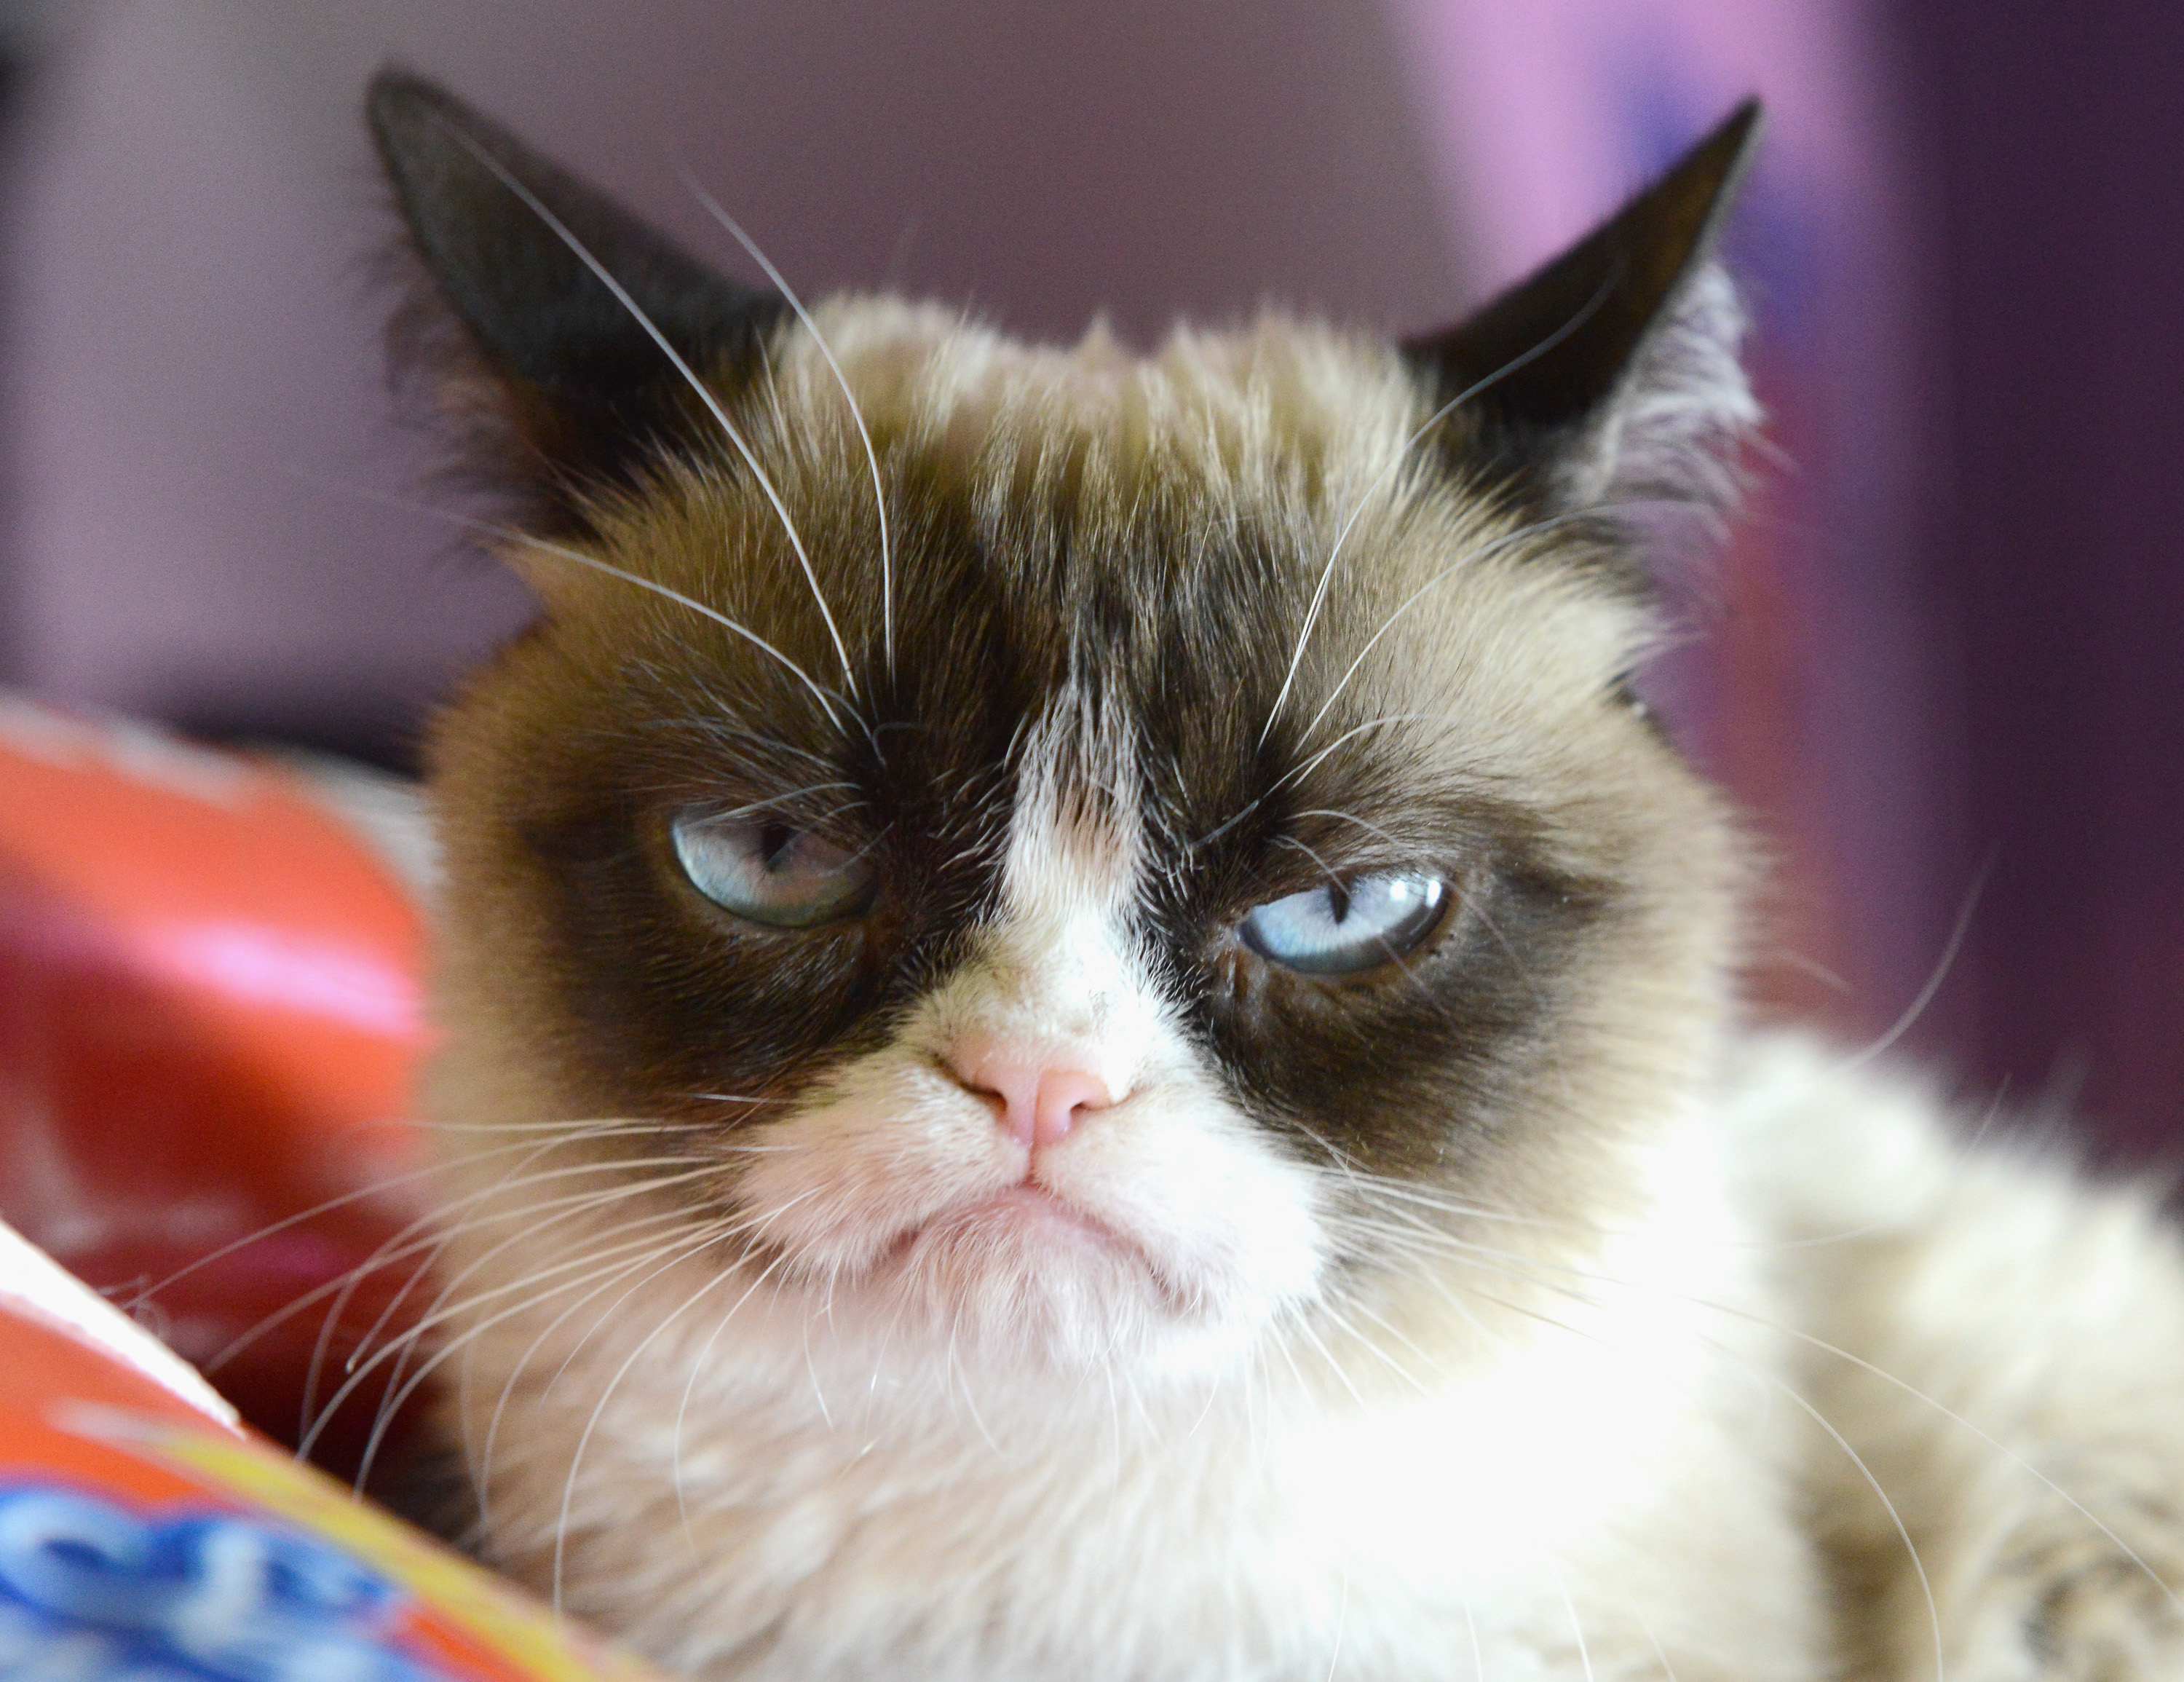
\includegraphics[width=0.75\linewidth]{image.jpg}|\\
\verb|	\caption{Dit is een voorbeeld van een figuur-float}|\\
\verb|	\label{fig:VoorbeeldFigFloat}|\\
\verb| \end{figure}|

 
 \begin{figure}[!ht]
 	\centering
 	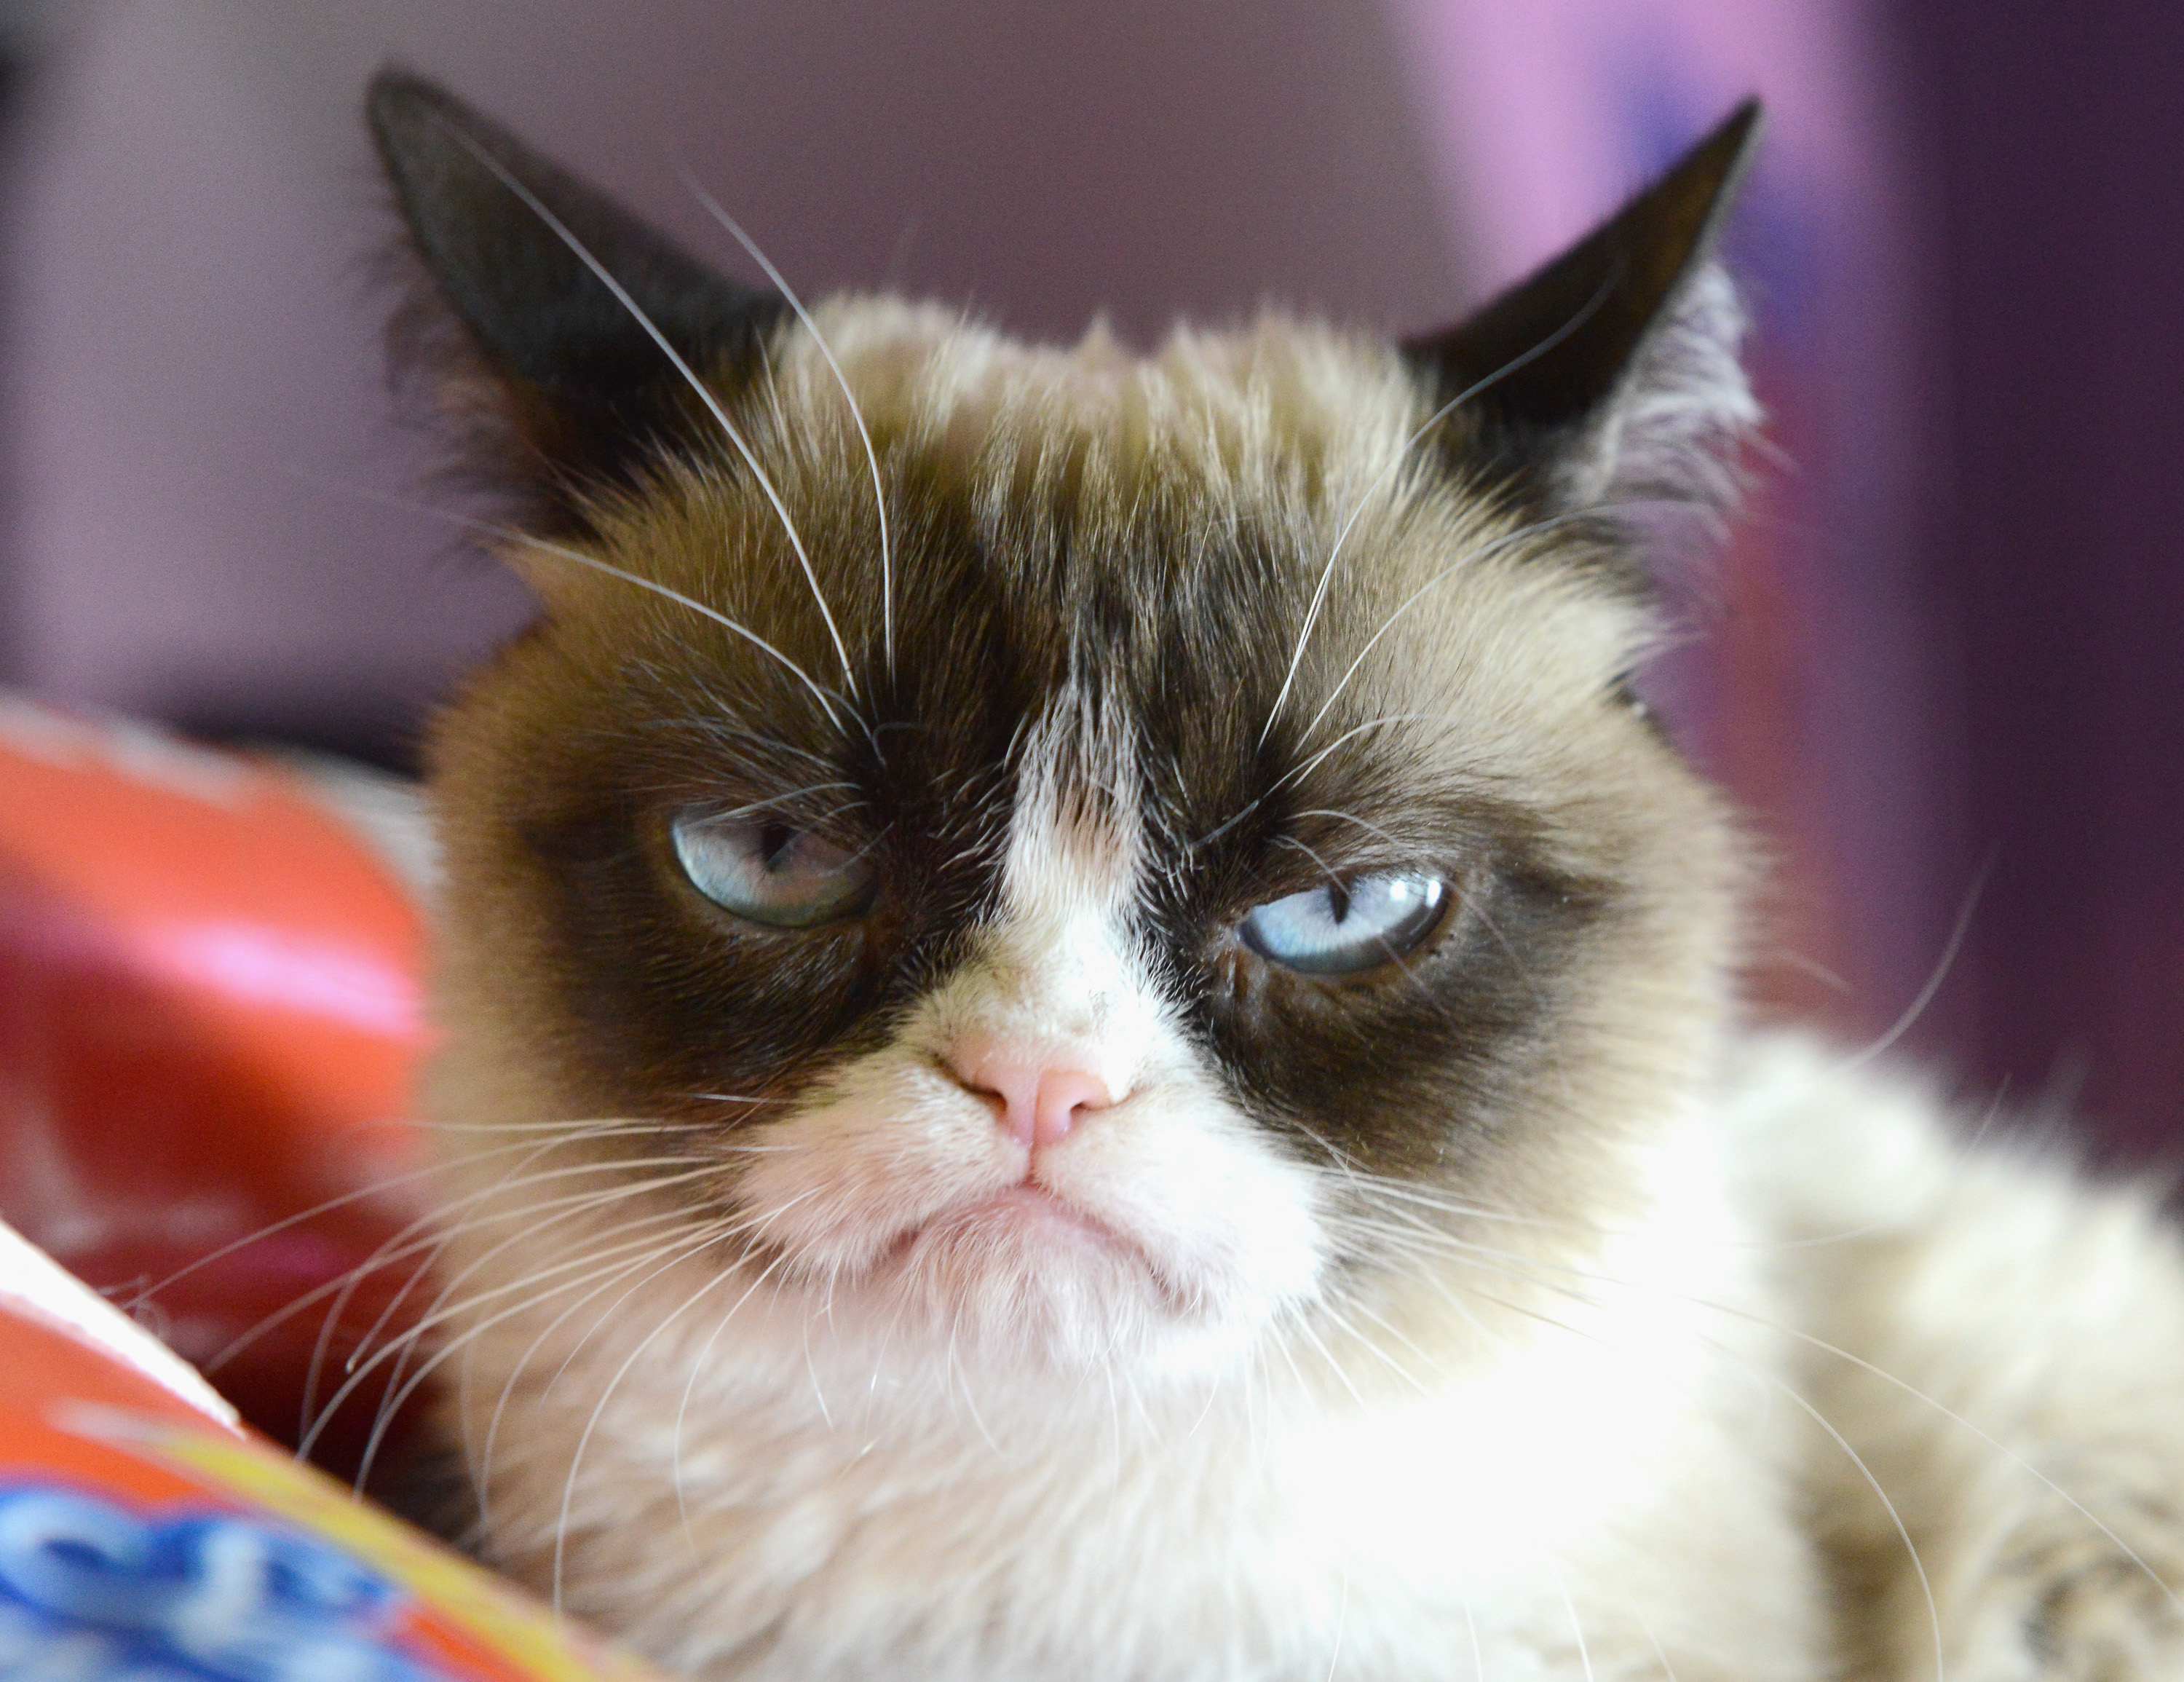
\includegraphics[width=0.75\linewidth]{image.jpg}
 	\caption{Dit is een voorbeeld van een figuur-float}
 	\label{fig:VoorbeeldFigFloat}
 \end{figure}

Tabellen worden links uitgelijnd op de bladzijde. Ook het bijschrift wordt links uitgelijnd en boven de tabel geplaatst. Na de tabelnummer volgt de beschrijving van de tabel. Tabel \ref{tab:VoorbeeldTableFloat} toont een voorbeeld van een eigen tabel. Vermijd om tabellen te kopie\"eren van andere werken, maar herwerk ze en plaats de nodige bronvermelding. De nodige syntax om tabel \ref{tab:VoorbeeldTableFloat} te generen wordt hieronder weergegeven:

\verb|\begin{table}[!ht]|\\
\verb|\caption{Dit is een voorbeeld van een tabel}|\\
\verb|\begin{tabular}{ccc}|\\
\verb|\hline|\\
\verb|Kolom 1 & Kolom 2 & Kolom 3\|\\
\verb|\hline|\\
\verb|1 & 2 & 3\\|\\
\verb|4 & 5 & 6\\|\\
\verb|\hline|\\
\verb|\end{tabular}|\\
\verb|\label{tab:VoorbeeldTableFloat}|\\
\verb|\end{table}|

Tot slot, let er op dat er expliciet naar elke tabel en figuur verwezen wordt vanuit de tekst. 

\begin{table}[!ht]
		\caption{Dit is een voorbeeld van een tabel}
	\begin{tabular}{ccc}
		\hline
		Kolom 1 & Kolom 2 & Kolom 3\\
		\hline
		1 & 2 & 3\\
		4 & 5 & 6\\
		\hline
	\end{tabular}
\label{tab:VoorbeeldTableFloat}
\end{table}
%%%%%%%%%%%%%%%%%%%%%%%%%%%%%%%%%%%%%%%%%%%%%%%%%%%%%%%%%%%%%%%%%%% 
%                                                                 %
%                            CHAPTER                              %
%                                                                 %
%%%%%%%%%%%%%%%%%%%%%%%%%%%%%%%%%%%%%%%%%%%%%%%%%%%%%%%%%%%%%%%%%%% 
\chapter{Richtlijnen voor formules}

Er zijn twee manieren om formules in LaTeX in te voeren:

\begin{itemize}
	\item Inline: $a^2+b^2 = c^2$ (\verb|$a^2+b^2 = c^2$|)
	\item In een equation omgeving 	(\verb|\begin{equation}	a^2+b^2 = c^2	\end{equation}|):
	\begin{equation}
		a^2+b^2 = c^2
	\end{equation}

\end{itemize}

Griekse letters geef je in d.m.b. het backslash commando. Bijvoorbeeld de letter sigma $\sigma$ verkrijg je door \verb|$\sigma$| inline in te geven. Dit is analoog voor griekse letters in de equation omgeving. Een beknopte lijst van symbolen vind je op de Wikibooks pagina voor LaTeX (\href{https://nl.wikibooks.org/wiki/LaTeX/Wiskundige_formules}{link}). Alle andere nuttige informatie omtrent het gebruik van LaTeX voor formules vind je hier ook terug.
\cleardoublepage
%%%%%%%%%%%%%%%%%%%%%%%%%%%%%%%%%%%%%%%%%%%%%%%%%%%%%%%%%%%%%%%%%%% 
%                                                                 %
%                            CHAPTER                              %
%                                                                 %
%%%%%%%%%%%%%%%%%%%%%%%%%%%%%%%%%%%%%%%%%%%%%%%%%%%%%%%%%%%%%%%%%%% 
\chapter{Richtlijnen voor referenties}

\section{Inleiding}
De referentielijst bevat de volledige lijst van literatuur en bronnen waarnaar in de tekst wordt verwezen. Door systematisch de referentielijst aan te vullen bij het schrijven van het literatuuroverzicht gaat er achteraf geen tijd verloren aan het opnieuw opzoeken van referenties.

\section{Referentiestijl}

Voor het verwijzen naar informatiebronnen wordt gebruik gemaakt van het numerisch systeem  of van het auteur-jaar systeem. Dit kies je door volgend commando in het latex bronbestand aan te passen:

\begin{itemize}
	\item numerisch (IEEE) : \verb|\bibliographystyle{ieee}|
	\item alfabetisch (APA) : \verb|\bibliographystyle{apalike}|
\end{itemize}

Plaats je bronnen in een \textit{bibtex} bestand (evt. via software zoals bv. Jabref Endnote of Mendeley), waarnaar je verwijst vanuit je thesis text a.d.h.v. het commando \verb|\cite|. Enkele links naar nuttige software in deze context:

\begin{itemize}
	\item \href{http://www.jabref.org/}{JabRef (Open Source)}
	\item \href{http://www.mendeley.com}{Mendeley (Freeware)}
	\item \href{http://www.endnote.com}{EndNote (Paid license)}
\end{itemize}

Indien je zelf een .bibtex bestand wil aanleggen dien je volgende syntax te volgen voor een tijdschriftartikel:
\clearpage
\verb|@article{hughes2005,|\\
\verb|title={Isogeometric analysis: CAD, finite elements, NURBS, exact geometry|\\ \verb|and mesh refinement},|\\
\verb|author={Hughes, Thomas JR and Cottrell, John A and Bazilevs, Yuri},|\\
\verb|journal={Computer methods in applied mechanics and engineering},|\\
\verb|volume={194},|\\
\verb|number={39},|\\
\verb|pages={4135--4195},|\\
\verb|year={2005},|\\
\verb|publisher={Elsevier}|\\
\verb|}|

Enkele voorbeelden van het gebruik van bronnen in een tekst (in APA stijl): 

Recent werd het Higgs boson experimenteel vastgesteld door Aad et al.\ \cite{aad2012} (syntax: \verb|\cite{aad2012}|). 

Als alternatief voor het discretiseren van een CAD model vooraleer een eindige elementenanalyse te kunnen toepassen, stellen Hughes et al.\ voor om de nodige elementenformulering rechtstreeks uit de NURBS beschrijving van de CAD geometrie te halen \cite{hughes2005} (syntax: \verb|\cite{hughes2005}|). Daarnaast introduceren ze tevens een k-iteratieve procedure als een verfijning van de geldende p- en h-iteratieve procedures in eindige elementen methoden \cite{cottrell2009} (syntax: \verb|\cite{cottrell2009}|).
% Bibliografie: referenties. De items zitten in bibliografie.bib
%%%%%%%%%%%%%%%%%%%%%%%%%%%%%%%%%%%%%%%%%%%%%%%%%%%%%%%%%%%%%%%%%
% Indien je ook de niet geciteerde werken in je bibliografie wil opnemen, commentarieer dan onderstaande regel uit!
%\nocite{*}
\bibliographystyle{apalike}
\bibliography{bibliografie}

% Eventueel enkele appendices
%%%%%%%%%%%%%%%%%%%%%%%%%%%%%%
\appendix
\chapter{Uitleg over de appendices}
Bijlagen worden bij voorkeur enkel elektronisch ter beschikking gesteld. Indien essentieel kunnen in overleg met de promotor bijlagen in de scriptie opgenomen worden of als apart boekdeel voorzien worden.

Er wordt wel steeds een lijst met vermelding van alle bijlagen opgenomen in de scriptie. Bijlagen worden genummerd het een drukletter A, B, C,...

Voorbeelden van bijlagen:\\
Bijlage A: \qquad	Detailtekeningen van de proefopstelling \\
Bijlage B: \qquad	Meetgegevens (op USB)
\\





% Back cover: change according to the correct campus

\includepdf{private/back_fiiw_denayer.pdf}
% 
\includepdf{private/back_fiiw_denayer_eng.pdf} % For the english version
%
\includepdf{private/back_fiiw_geel.pdf}
% 
\includepdf{private/back_fiiw_geel_eng.pdf} % For the english version
%
\includepdf{private/back_fiiw_gent.pdf}
% 
\includepdf{private/back_fiiw_ghent_eng.pdf} % For the english version
%
\includepdf{private/back_fiiw_brugge.pdf}
% 
\includepdf{private/back_fiiw_bruges_eng.pdf} % For the english version
%
\includepdf{private/back_fiiw_groept.pdf}
% \includepdf{private/back_fiiw_groupt_eng.pdf} % For the english version

\end{document}
